\chapter{From First Commission to Brokerage Ownership}

This interview contains no blackboard derivation, but it does have a clean quantitative spine. We move from an opening money shock, to the accumulation of a real-estate skill stack, to the threshold logic of brokerage, to the arithmetic of wholesaling, partnership, and downside risk. The right way to read it is not as a bag of motivational lines, but as a sequence of increasingly structured economic moves: first a paycheck, then a commission, then a platform, then contract control, and finally long-horizon judgment.

\section{Opening Shock: Money Appears in Jumps}

We begin where the lecture begins: not with credentials, but with scale. A novice sits in a brokerage office and watches a local operator receive a \(\$200{,}000\) check. A few sentences later the scene collapses to wage life: pizza delivery, mopping floors, a first phone call, and a first closing worth roughly \(\$6{,}000\) to \(\$7{,}000\).

\paragraph{Anecdote.}
The opening is memorable because it is discontinuous. One does not move gradually from a \(\$600\) paycheck to the idea of a \(\$200{,}000\) closing. One sees the larger number first, then reinterprets one's own economic life.

\paragraph{Claim.}
The lecture's first claim is that entrepreneurship often becomes believable through an income shock rather than through a careful forecast. The first commission is not merely extra money; it changes the perceived size of the game.

\paragraph{Mechanism.}
If we write the first closing as \(F\) and the earlier paycheck scale as \(W\), then the motivational discontinuity is the ratio
\begin{align}
F &\approx 6{,}000 \text{ to } 7{,}000, \\
W &\approx 600, \\
R_{\mathrm{shock}} &= \frac{F}{W} \approx 10 \text{ to } 11.7 .
\end{align}
Even if we compare the closing to a larger full-time paycheck scale of roughly \(\$1{,}500\) to \(\$2{,}000\), we still obtain a multiple rather than an increment:
\begin{equation}
\frac{6{,}000}{2{,}000}=3,
\qquad
\frac{7{,}000}{1{,}500}\approx 4.7 .
\end{equation}
That is the basic rhythm of the opening: money appears in jumps, and the jump itself motivates the rest of the chapter.

\section{Building the Skill Stack Before Ownership}

After the cold open, the interview resets and gives us the long route to the present. The speaker does not present ownership as a single clever move. He presents it as accumulation.

\paragraph{Anecdote.}
The sequence is concrete and chronological: born in Cleveland, raised in Austin, influenced by a mother who showed what real estate could make possible, licensed at \(17\), educated in real estate finance, trained in appraisal and apartments, later building and selling a management company, and finally building an entrepreneurial brokerage with a longtime childhood friend.

\paragraph{Claim.}
The lecture's second claim is that ownership grows out of layered contact with the business. Sales, appraisal, management, graduate study, and operating experience are not decorative credentials. They are different views of the same asset class.

\paragraph{Mechanism.}
A compact way to keep the scale markers in view is the following list:
\begin{itemize}
\item License obtained at age \(17\).
\item Management company built to roughly \(700\) doors.
\item Later property ownership described as roughly \(130\) properties.
\end{itemize}
The important point is not numerical vanity. The point is that the interview keeps moving from access to responsibility: first learning how deals happen, then learning how assets are valued, then learning how operations work, and only then trying to own the platform itself.

\section{College, Credentials, and Network Value}

The host now asks a natural question: if formal schooling is part of the story, is it necessary for success?

\subsection{Question \& Answer}

\paragraph{Question.}
Is college necessary for success in business and in real estate? And, even if it is not necessary, was it transferable?

\paragraph{Answer.}
The answer given in the interview is deliberately non-binary. College is not presented as strictly necessary. But neither is it dismissed. Its value depends on what one makes of it. The speaker's emphasis falls not on the diploma alone, but on the environment: a room full of people interested in business, all of whom could help one another for years if they actually coordinated.

\paragraph{Mechanism.}
The lecture is careful here. Credentials matter in at least two ways:
\begin{itemize}
\item They can satisfy formal requirements, as later happens with broker-related coursework.
\item They can place one inside a network of peers whose ambition is not yet organized.
\end{itemize}
So the educational question is reframed. The issue is not simply whether one sits in class. The issue is whether one converts a shared institutional setting into future business cooperation.

\begin{remark}
This is a useful place to resist overcompression. The lecture does not say merely, ``college is unnecessary.'' It says something more precise: institutional value is contingent on how aggressively we use the people and opportunities around us.
\end{remark}

\section{First Entry, First Deal, First Real Money}

The interview now rewinds, explicitly, to the beginning. We are asked not for the current platform but for the first mechanism of entry.

\subsection{Question \& Answer}

\paragraph{Question.}
How did the first involvement in real estate actually happen, and what was the first money?

\paragraph{Answer.}
The speaker did what many beginners do: he interviewed with brokerages while thinking the brokerage held all the power. The surprise is that the market is partly the reverse. New agents are wanted. In the interview, that misunderstanding is corrected dramatically by a mentor figure who receives a \(\$200{,}000\) check in front of the novice and says, in effect, that one can get there too.

\paragraph{Anecdote.}
The next move is equally important. The speaker takes the brokerage opportunity but continues delivering pizza because cash flow is still needed. Then the first real-estate call arrives while he is mopping the floor. He drops the mop, takes the call, closes the deal, and sees a check that no previous paycheck had prepared him for.

\paragraph{Mechanism.}
If we compare the first closing to the wage scale that structured his earlier life, we see why the episode becomes decisive:
\begin{equation}
\frac{6{,}000}{600}=10,
\qquad
\frac{7{,}000}{600}\approx 11.7.
\end{equation}
The point is not that one commission guarantees a career. The point is that a single transaction can reset the imagination. The interview keeps returning to this kind of discontinuity: the market is larger than the beginner initially thinks.

\section{From Agent to Broker: Thresholds and Platform Economics}

Once the first-deal story is complete, the interview scales up from entry to structure. How does one move from being an agent inside someone else's system to becoming the broker who carries responsibility for others?

\subsection{Question \& Answer}

\paragraph{Question.}
What changes when an agent becomes a broker?

\paragraph{Answer.}
The answer has two layers. First, there is threshold logic: time, transactions, points, and coursework. Second, there is institutional burden: the broker becomes the party who is responsible, who is on the hook, who trains, and who supports.

\begin{definition}[Broker in the interview sense]
A broker is not just a higher-paid salesperson. In the lecture, the broker is the supervisory licensed party under whom agents operate, and the one who carries legal and operating responsibility for the platform.
\end{definition}

We can compress the spoken threshold structure into the following symbolic form:
\begin{equation}
Y_{\mathrm{req}} = 4 \text{ years},
\qquad
P_{\mathrm{req}} \approx 900 .
\end{equation}
The lecture also notes an earlier regime with a shorter time requirement:
\begin{equation}
Y_{\mathrm{req}}^{\mathrm{old}} = 2 \text{ years},
\qquad
Y_{\mathrm{req}}^{\mathrm{new}} = 4 \text{ years}.
\end{equation}

\begin{table}[h]
\centering
\begin{tabular}{p{0.28\linewidth}p{0.58\linewidth}}
\textbf{Spoken threshold} & \textbf{Interview description} \\
Experience & Formerly two years; later changed to four years \\
Transaction logic & A point system, stated at roughly \(900\) points \\
Education & Required credit hours; the speaker says college and master's work satisfied these \\
Institutional change & The broker is responsible, trains agents, supports them, and remains on the hook \\
\end{tabular}
\caption{Transcript-based summary of the move from agent to broker.}
\end{table}

The interview then turns immediately to platform economics. If \(C\) denotes gross commission on a closed deal, the current and earlier split structures can be written as
\begin{align}
C_{\mathrm{agent}} &= 0.9\,C,
&
C_{\mathrm{brokerage}} &= 0.1\,C,
\\
C_{\mathrm{agent}}^{\mathrm{old}} &= 0.5\,C,
&
C_{\mathrm{brokerage}}^{\mathrm{old}} &= 0.5\,C.
\end{align}
This is not a mere pricing detail. It says what kind of platform the firm is trying to be.

\paragraph{Worked example.}
Take a gross commission of \(C=10{,}000\). Then
\begin{equation}
C_{\mathrm{agent}}^{90/10}=9{,}000,
\qquad
C_{\mathrm{agent}}^{50/50}=5{,}000.
\end{equation}
So the agent's gross share under the \(90\text{--}10\) model is
\begin{equation}
\frac{0.9C}{0.5C}=1.8
\end{equation}
times the agent's gross share under the older \(50\text{--}50\) model. The lecture uses this contrast to show that brokerage is not only licensing structure but also platform design.

\section{Leadership Burden and the Logic of Partnership}

Once brokerage has been explained formally, the interview asks what it feels like in practice. The first answer is not freedom. It is strain.

\paragraph{Anecdote.}
The speaker lists the familiar disorder of operating life: deals falling apart, lawsuits, complaints, and the need to lead while carrying private challenges that may not be visible to the team.

\paragraph{Claim.}
The lecture's claim here is that ownership is not only upside. It is the obligation to maintain coherence under pressure. That is why the next question, about partnership, matters so much.

\subsection{Question \& Answer}

\paragraph{Question.}
What should one look for in a business partner?

\paragraph{Answer.}
The answer is severe before it becomes optimistic. The speaker says that perhaps only one partnership in twenty works out. So the problem is not to praise partnership in the abstract, but to explain why this one did.

\paragraph{Mechanism.}
The lecture gives a sequence of tests:
\begin{itemize}
\item A long personal history rather than a fresh transactional relationship.
\item A period of distrust grounded in the partner's earlier life.
\item Repeated evidence of overperformance: if told to knock \(10\) doors, he knocks \(100\); if told to call a certain number of people, he calls many more.
\item A durable change in habits: sobriety, discipline, early rising, meditation, work.
\item Clear role division once trust is earned.
\end{itemize}

The eventual division is not vague. It is operational:
\begin{itemize}
\item The implementer handles money, profitability, hiring, firing, and execution.
\item The visionary handles networking, relationships, and new ideas.
\end{itemize}
The lecture names this framework through the language of \emph{Traction}. The important point for the notes is not the brand name by itself, but the complementarity: the firm becomes more stable when strategic imagination and daily execution are not confused.

\section{Biggest Deal, Downside, and Long-Horizon Judgment}

By the time we reach the financial section, the interview has already built the necessary scaffolding: first entry, licensing, brokerage, leadership, and partnership. Now it can speak about large transactions without making them sound like isolated luck.

\subsection{Question \& Answer}

\paragraph{Question.}
What was the biggest deal, and how did it work?

\paragraph{Answer.}
The answer is a wholesaling story. In the lecture's account, a property is put under contract at one price, control over that contract is secured through earnest and option money, and then a higher-value buyer is found. The spread between the two prices becomes the economic core of the deal.

\begin{definition}[Wholesale spread]
In the narrow sense used in this interview, we place a property under contract at price \(V_{\mathrm{contract}}\), preserve control of that contract, and later monetize that control at a higher effective exit value \(V_{\mathrm{exit}}\). The gross spread is
\begin{equation}
S = V_{\mathrm{exit}} - V_{\mathrm{contract}} .
\end{equation}
\end{definition}

The spoken deal numbers are approximately
\begin{equation}
V_{\mathrm{contract}} \approx 2.0\,\mathrm{M},
\qquad
V_{\mathrm{exit}} \approx 2.7\,\mathrm{M},
\qquad
E_{\mathrm{earnest+option}} \approx 20{,}000 .
\end{equation}

\begin{figure}[h]
\centering
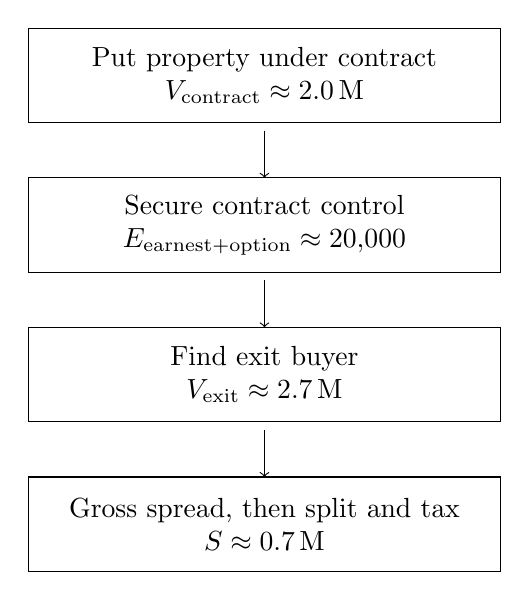
\begin{tikzpicture}[x=1cm,y=1cm]
\draw (0,0) rectangle (6,1.2);
\node[align=center] at (3,0.6)
{Put property under contract\\
$V_{\mathrm{contract}} \approx 2.0\,\mathrm{M}$};

\draw[->] (3,-0.1) -- (3,-0.7);

\draw (0,-1.9) rectangle (6,-0.7);
\node[align=center] at (3,-1.3)
{Secure contract control\\
$E_{\mathrm{earnest+option}} \approx 20{,}000$};

\draw[->] (3,-2.0) -- (3,-2.6);

\draw (0,-3.8) rectangle (6,-2.6);
\node[align=center] at (3,-3.2)
{Find exit buyer\\
$V_{\mathrm{exit}} \approx 2.7\,\mathrm{M}$};

\draw[->] (3,-3.9) -- (3,-4.5);

\draw (0,-5.7) rectangle (6,-4.5);
\node[align=center] at (3,-5.1)
{Gross spread, then split and tax\\
$S \approx 0.7\,\mathrm{M}$};
\end{tikzpicture}
\caption{Transcript-based schematic of the wholesale transaction described in the interview.}
\end{figure}

\paragraph{Worked derivation.}
We can now write the basic arithmetic in the order the interview suggests:
\begin{align}
S &= V_{\mathrm{exit}} - V_{\mathrm{contract}}, \\
&\approx 2.7\,\mathrm{M} - 2.0\,\mathrm{M}, \\
&= 0.7\,\mathrm{M}.
\end{align}
This matches the repeated \(\$700{,}000\) scale in the interview, though the speaker also mentions \(\$780{,}000\), so we should keep the number approximate.

There is a second lesson here: a comparatively small amount of upfront money controls a much larger contract value. If we define the contract-control leverage by
\begin{equation}
L_{\mathrm{control}}
=
\frac{V_{\mathrm{contract}}}{E_{\mathrm{earnest+option}}},
\end{equation}
then the spoken numbers give
\begin{equation}
L_{\mathrm{control}}
\approx
\frac{2{,}000{,}000}{20{,}000}
=100.
\end{equation}
This is not debt leverage in the narrow banking sense. It is contract-control leverage: a small amount of cash secures decision rights over a much larger asset pathway.

\begin{remark}
The lecture uses the phrase ``actual ownership'' for control of the contract. We should state this cautiously. Economically, the point is control over the paper and therefore over a potential spread, not necessarily full fee-simple ownership in the strongest legal sense.
\end{remark}

The speaker then adds a useful correction. Headline numbers overstate realized wealth. The gross figure must still pass through partner splits, taxes, and any separate commission structure.

\begin{table}[h]
\centering
\begin{tabular}{p{0.42\linewidth}p{0.38\linewidth}}
\textbf{Layer} & \textbf{Approximate interview number} \\
Gross spread headline & \(\$700{,}000\) scale, with \(\$780{,}000\) also mentioned \\
Equal split across three partners & about \(\$233{,}333\) to \(\$260{,}000\) each before tax \\
Separate commission & \(3\%\) is mentioned, but its exact relation to the spread is unclear \\
Tax effect & described as materially reducing the retained amount \\
\end{tabular}
\caption{Gross-to-net logic of the biggest deal, kept approximate because the spoken numbers are not perfectly stable.}
\end{table}

\subsection{Question \& Answer}

\paragraph{Question.}
What were the best and worst financial decisions?

\paragraph{Answer.}
The worst decision, by the speaker's own account, was cannabis stock. The best decision was partnership with Alex. The lecture therefore places a speculative capital loss and a social-organizational success side by side.

\paragraph{Mechanism.}
The downside is described in stark daily terms:
\begin{align}
\Delta V_{\mathrm{day}} &\approx -(60\text{k to }100\text{k}), \\
R_q &\approx 67\,\mathrm{M},
\qquad
M \approx 40\,\mathrm{M}.
\end{align}
If we compress the speaker's own valuation intuition into simple ratios, we obtain
\begin{equation}
\frac{M}{R_q} \approx \frac{40}{67} \approx 0.60,
\qquad
\frac{M}{4R_q} \approx \frac{40}{268} \approx 0.15.
\end{equation}
These are not endorsed valuation formulas for the chapter. They are the arithmetic behind the speaker's claim that the market is undervaluing the business and that the position is therefore ``early'' rather than simply broken.

\paragraph{Claim.}
The deeper lesson is more stable than the trade. The interview finally says that the best financial decision was not a stock pick at all, but a partner selection. In other words, organization can dominate speculation.

\paragraph{Closing movement.}
The final minutes widen the frame once more. The interview recounts bizarre field stories, returns to long-horizon vision, and ends not on a deal metric but on a goal: to build something coherent enough that agents say their lives were changed by it. We have moved a long way from the opening \(\$200{,}000\) check. Money remains central, but it has been absorbed into platform design, role design, and mission.

\section{Summary}

The lecture begins with a money shock and ends with a theory of entrepreneurial structure. In between, it unfolds a sequence that we can state compactly:

\begin{itemize}
\item A first large observed number changes the scale of ambition.
\item A layered skill stack makes ownership intelligible.
\item College is useful when it is converted into relationships and coordinated practice.
\item Brokerage is a threshold system: years, points, classes, and responsibility.
\item Platform economics matter, as shown by the difference between \(90\text{--}10\) and \(50\text{--}50\).
\item Partnership works only when trust, discipline, and role complementarity are repeatedly demonstrated.
\item Large deals are not just large numbers; they are spreads, control rights, splits, and taxes.
\item Long-run judgment is finally social as much as financial: the right partner may be the best trade in the whole lecture.
\end{itemize}

That is the chapter's central mathematical and narrative idea. We do not merely chase bigger checks. We move from isolated income events to repeatable structures of control, responsibility, and judgment.